% capitulos/cap2.tex — Capítulo 2 (Referencial Teórico).
% Reescrito em 25/09/2026 no enxugamento pós-feedback (ver
% auditoria/plano_enxugamento.md). Passa a concentrar a literatura que antes
% se repetia entre a Introdução (seção 1.1) e a Metodologia (seção 3.1,
% "Os cinco elementos que delimitam a lacuna"): cada evidência aparece uma
% vez, aqui, e os demais capítulos remetem a ela. Números e citações
% conferidos contra a versão anterior (auditoria/versoes/pre_enxugamento/).
% Modelagem conceitual (robinson2008a/b) saiu deste capítulo e é citada em
% uma frase no Passo 3 (cap3.tex), onde é usada. Contém: 1 Figura
% (fig:as-is) e 2 equações numeradas (eq:pl, eq:milp), vindas do Cap. 3.
\chapter{Referencial Teórico}

Este capítulo reúne a literatura que sustenta o trabalho. A seção~\ref{sec:po-barreira} apresenta a Pesquisa Operacional e a barreira que dificulta seu uso nas organizações. A seção~\ref{sec:nl2opt} descreve como os modelos de linguagem passaram a ser usados para formular problemas de otimização. A seção~\ref{sec:lacunas} mostra o que essas propostas ainda não resolvem. A seção~\ref{sec:autocorrecao} trata de um limite dos modelos de linguagem que orienta o desenho do artefato: a dificuldade de encontrar os próprios erros. A revisão sistemática da literatura, cujo protocolo está na seção~\ref{sec:revisao}, será executada no TG2 e ampliará este capítulo.

\section{Pesquisa Operacional e a barreira da modelagem}
\label{sec:po-barreira}

A Pesquisa Operacional (PO) aplica métodos científicos a problemas de decisão e de alocação de recursos \cite{arenales2007}. Seu principal instrumento é a otimização matemática, que descreve a decisão por variáveis, o critério de escolha por uma função objetivo e os limites da operação por restrições. Este trabalho trata de duas classes de modelo. Na programação linear (PL), todas as variáveis são contínuas, como na forma padrão~\eqref{eq:pl}. Na programação linear inteira mista (PLIM), parte das variáveis assume apenas valores inteiros, como em~\eqref{eq:milp} \cite{arenales2007}:

\begin{align}
  \min \quad & c'x \notag \\
  \text{s.a.} \quad & Ax \geq b \label{eq:pl} \\
  & x \geq 0 \notag
\end{align}

\begin{align}
  \min \quad & c'x + d'y \notag \\
  \text{s.a.} \quad & Ax + Gy \geq b \label{eq:milp} \\
  & x \geq 0,\ y \geq 0 \text{ e inteiro} \notag
\end{align}

em que $x$ é o vetor de variáveis contínuas, $y$ o vetor de variáveis inteiras, $c$ e $d$ os vetores de coeficientes da função objetivo, $A$ e $G$ as matrizes de coeficientes das restrições e $b$ o vetor dos termos independentes.

A otimização é empregada em cadeias de suprimentos, saúde, energia e infraestrutura, com benefícios econômicos e sociais relevantes \cite{wasserkrug2025}. Sua adoção nas organizações, porém, esbarra há décadas no mesmo obstáculo. No final da década de 1970, desenvolvedores de um sistema comercial de programação linear já avaliavam que resolver o modelo não era a barreira principal: gerenciar os dados, formular e construir o modelo, analisar e comunicar os resultados custava muito mais (Krabek; Sjoquist; Sommer, 1980 \textit{apud} \citeauthor{fourer2012}, \citeyear{fourer2012}, p.~1). A literatura de implementação da mesma época atribui parte das falhas à comunicação deficiente entre gestores e analistas \cite{henderson1980}.

O diagnóstico se repete em diferentes setores. \citeonline{langabeer2010} discutem a difusão limitada da PO na gestão hospitalar. \citeonline{lai2013} concluem que, em organizações logísticas, a competência das pessoas e a reorganização dos processos pesam mais do que o investimento financeiro na adoção de ferramentas de PO. O perfil dos usuários confirma a barreira: 81\% dos usuários do \textit{solver} comercial Gurobi têm pós-graduação e, destes, 49\% são formados em Pesquisa Operacional \cite[p.~1]{ahmaditeshnizi2026}. \citeonline{shobrys2002} acrescentam que os resultados da otimização só são aceitos quando a técnica e seus usuários têm credibilidade junto à gerência; na programação da produção, por isso, a prática ainda recorre à simulação.

O retrato mais detalhado da prática de modelagem é o de \citeonline{lawless2025}, que entrevistaram quinze desenvolvedores de modelos de otimização de setores como manufatura, saúde, logística, defesa e educação. Os autores descrevem um fluxo de seis estágios --- elicitação do problema, tratamento dos dados, desenvolvimento do modelo, implementação, validação e implantação --- percorrido com idas e vindas, e não em linha reta \cite[p.~6]{lawless2025}. Três gargalos desse fluxo interessam a este trabalho:

\begin{enumerate}[label=\alph*)]
  \item na elicitação, as descrições iniciais do problema costumam ser vagas, informais ou contraditórias, e só se tornam um problema de decisão consistente após várias rodadas entre o modelador e quem conhece a operação;
  \item o tratamento dos dados é o estágio mais custoso, com até 70\% do esforço do projeto, e os dados disponíveis podem obrigar a refazer a formulação \cite[p.~15]{lawless2025};
  \item a validação é manual e depende de convencer as partes interessadas; quando os elementos que sustentam a recomendação não ficam visíveis, a otimização é percebida como uma ``caixa mágica'', poderosa porém opaca.
\end{enumerate}

A Figura~\ref{fig:as-is} resume esse fluxo. O problema que ela evidencia é estrutural, e não de competência: o conhecimento do problema fica com o gestor e o domínio do formalismo fica com o especialista. Cada passagem de um para o outro gera espera e pode distorcer a intenção original da decisão.

\begin{figure}[htbp]
\caption{Cenário \textit{as is}: fluxo de modelagem de otimização com transferência entre gestor e especialista}
\label{fig:as-is}
\centering
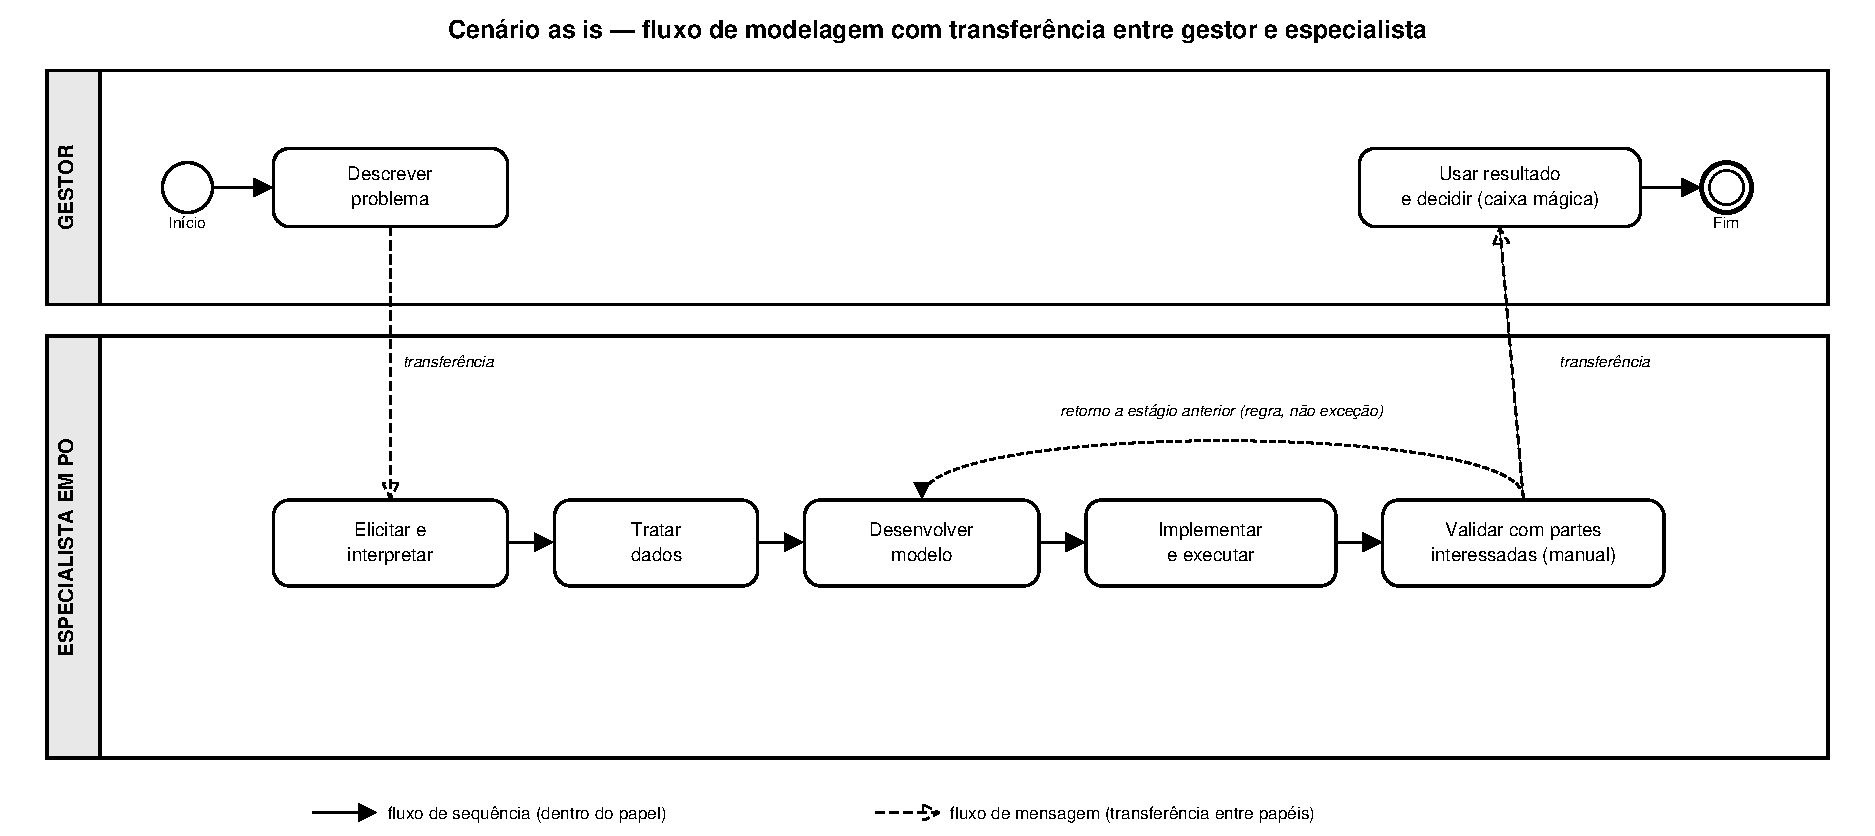
\includegraphics[width=0.95\textwidth]{figuras/fig1_as_is.pdf}
\fontenota{elaborado pelo autor com base em \citeonline{lawless2025} e em notação BPMN conforme \citeonline{dumas2018}}
\end{figure}

O próprio estudo de \citeonline[p.~19]{lawless2025} declara seu limite principal: foram entrevistados apenas especialistas, e as questões de acessibilidade e usabilidade para não especialistas, assim como a perspectiva dos gestores que usam os resultados, ficaram fora do escopo. A lacuna investigada aqui é, portanto, uma agenda deixada em aberto por quem descreveu a prática com mais detalhe.

Resta saber quando a otimização é o instrumento adequado. \citeonline[p.~761]{rosenhead2006} recupera as condições sob as quais a análise tradicional de PO funciona bem: organização estruturada em hierarquia definida; poucos membros analiticamente sofisticados; tarefa bem definida e repetitiva, que gera dados confiáveis; e consenso sobre as prioridades (Greenberger; Crenson; Crissey, 1976 \textit{apud} \citeauthor{rosenhead2006}, \citeyear{rosenhead2006}, p.~761). Onde há muitos atores, interesses em conflito e incertezas difíceis de representar, o instrumento indicado são os métodos de estruturação de problemas, e não um modelo de otimização, automatizado ou não \cite{rosenhead2006}. Este trabalho se restringe às situações que atendem àquelas condições.

\section{Modelos de linguagem e formulação de otimização}
\label{sec:nl2opt}

Os modelos de linguagem de grande porte (\textit{Large Language Models}, LLMs) interpretam texto, geram representações estruturadas e produzem código. Por isso passaram a ser estudados como ponte entre a descrição de um problema e seu modelo matemático, tarefa chamada \textit{Natural Language to Optimization} (NL2Opt). A área ganhou agenda própria em 2022, com a competição NL4Opt, realizada na conferência NeurIPS, que formalizou a tarefa e publicou um conjunto de dados de referência \cite{ramamonjison2023}. Esse conjunto, o LPWP, reúne 1101 problemas anotados de seis domínios, repartidos em 713 de treinamento, 99 de desenvolvimento e 289 de teste \cite{ramamonjison2023}; são enunciados autocontidos, tipicamente com duas a três variáveis e valores numéricos explícitos no próprio texto \cite{mostajabdaveh2024}.

Desde então surgiram abordagens que automatizam partes diferentes do processo. \citeonline{li2023} propuseram um processo em três fases, que identifica as variáveis, classifica objetivo e restrições e gera o modelo de PLIM. \citeonline{mostajabdaveh2024} desenvolveram uma arquitetura multiagente voltada à formulação e à verificação. O OptiMUS formula modelos, gera e depura código e executa \textit{solvers} \cite{ahmaditeshnizi2024, ahmaditeshnizi2026}. \citeonline{astorga2025} trataram a formulação como busca em um espaço de hipóteses de modelagem. OptiTrust e OptiAgent acrescentaram geração de dados verificáveis, agentes especializados e ciclos de correção \cite{lima2025, monteiro2026}.

O OptiAgent \cite{monteiro2026} é o trabalho mais próximo desta proposta. Ele organiza seis agentes sobre um estado compartilhado, com quatro laços de correção e limite de três iterações por laço. Ao menos um laço foi acionado em 27,8\% dos problemas do ComplexOR, 33,1\% do NLP4LP, 55,1\% do LogiOR e 61,4\% do IndustryOR \cite[p.~9]{monteiro2026}. Os autores atribuem os ganhos à divisão da tarefa entre agentes, e não à redação das instruções, e registram duas limitações: cada configuração foi executada uma única vez, sem medir a variabilidade das saídas; e a avaliação isolada de cada agente, assim como a avaliação com usuários não especialistas, ficou como trabalho futuro \cite[p.~11]{monteiro2026}. Medir o efeito isolado de um agente validador é justamente o experimento central deste trabalho.

\section{O que as propostas atuais não resolvem}
\label{sec:lacunas}

Cinco limitações do estado atual definem a lacuna deste trabalho. Nenhuma é inédita isoladamente; o que não se encontrou foi um artefato que trate as cinco em conjunto. No Capítulo 3, cada uma se converte em um requisito de projeto.

\textbf{Usuário.} As propostas se dirigem a quem já domina o formalismo. O OptiMUS-0.3 se apresenta como ferramenta de produtividade para profissionais que conhecem o domínio, reconhecem que o problema cabe em um modelo de PL ou PLIM e conseguem descrevê-lo com precisão; transformar problemas vagos ou incompletos em especificações concretas é, para os próprios autores, questão em aberto \cite{ahmaditeshnizi2026}. O copiloto de decisão proposto por \citeonline{wasserkrug2025}, capaz de dialogar com decisores e produzir modelos verificáveis sem exigir domínio de otimização, é apresentado como visão a alcançar, e não como resultado obtido.

\textbf{Fluxo completo.} Os sistemas cobrem partes do fluxo, em geral da leitura do enunciado à execução do \textit{solver}. O tratamento dos dados, estágio mais custoso da prática, é o menos automatizado, e a explicação ao decisor aparece como saída de texto, e não como etapa com requisitos próprios.

\textbf{Dados.} Nas organizações, os dados já existem antes do modelo: estão em planilhas e extrações de sistemas, com nomes de coluna em vocabulário de negócio, unidades próprias e granularidade que ninguém escolheu pensando em otimizar. Os conjuntos de avaliação recentes já separam a descrição dos valores numéricos --- o NLP4LP reúne 354 problemas, cada um com arquivo de dados, além de sete estudos de caso \cite[p.~7]{ahmaditeshnizi2026} ---, mas o arquivo é construído para a instância. No OptiMUS-0.3, o formato do arquivo é deduzido dos parâmetros extraídos do texto, e o usuário carrega os dados nesse formato ou usa dados gerados aleatoriamente \cite{ahmaditeshnizi2026}. O dado se ajusta ao modelo, e não o contrário. A dificuldade também não é de volume: no caso \textit{Amazon Locker}, o sistema manteve 100\% de formulações corretas em oito níveis de escala, de 3 KB a 935 KB \cite{ahmaditeshnizi2026}. O que falta é associar a grandeza citada no texto à coluna do arquivo que a contém.

\textbf{Idioma.} Os sistemas e conjuntos de avaliação da área foram desenvolvidos em inglês. O principal conjunto multilíngue de raciocínio matemático, o MGSM, traduz 250 problemas para dez idiomas, entre os quais não está o português; e o raciocínio intermediário em inglês frequentemente iguala ou supera o raciocínio no idioma da pergunta \cite{shi2023}. Não se pode supor, portanto, que resultados obtidos em inglês se transfiram para descrições organizacionais em português.

\textbf{Confiabilidade e rastreabilidade.} Código que executa e valor objetivo correto não garantem modelo correto. No exemplo de \citeonline{refai2025}, uma formulação recuperou duas das quatro restrições de referência, omitiu as de integralidade e de capacidade, acrescentou uma restrição inexistente no gabarito e ainda assim atingiu \textit{optimality gap} igual a zero: precisão de 0,67, revocação de 0,50 e erro aparente nulo. O estudo cobre apenas quatro problemas; mostra que o fenômeno existe, mas não com que frequência ocorre. Os próprios gabaritos também falham: na inspeção de \citeonline{xiao2025}, com cada caso validado por ao menos três especialistas, todos os conjuntos de avaliação, exceto o EasyLP, apresentaram erro em mais de 15\% dos problemas, chegando a pelo menos 54\% no IndustryOR. Como as correções automáticas são frequentes (seção~\ref{sec:nl2opt}), o usuário só consegue confiar no resultado se as premissas, os componentes do modelo, as validações e as correções ficarem registrados. Essa rastreabilidade do processo é diferente de expor o texto de raciocínio do modelo de linguagem: a primeira é verificável, porque incide sobre artefatos guardados e comparáveis com a saída final; o segundo não guarda relação garantida com o que foi efetivamente gerado.

\section{Autocorreção e verificação externa em modelos de linguagem}
\label{sec:autocorrecao}

\citeonline{tyen2024} separaram duas capacidades que costumavam ser tratadas juntas: encontrar um erro e corrigi-lo. Os modelos de linguagem testados falharam em localizar erros lógicos, mesmo em casos objetivos; mas, quando recebiam a localização do erro, corrigiam-no bem nas cinco tarefas de raciocínio avaliadas. O gargalo está em localizar, e não em corrigir.

O resultado confirma um diagnóstico anterior. \citeonline{huang2024} mostraram que, em tarefas de raciocínio, os modelos não melhoram ao revisar a própria resposta sem ajuda externa, e podem até piorar. Mostraram também que trabalhos que relatavam ganho usavam a resposta correta para decidir quando parar a revisão, o que não é autocorreção de fato. Em revisão crítica da área, \citeonline{kamoi2024} não encontraram trabalho que demonstre autocorreção bem-sucedida apoiada só na avaliação do próprio modelo.

Uma ressalva: treinamentos específicos e modelos de raciocínio mais recentes já mostram melhor capacidade de autoverificação, de modo que esse limite não é permanente. Para o modelo de uso geral empregado neste trabalho, a consequência de projeto é direta: um verificador deve localizar o erro com sinais externos ao modelo e entregar essa localização para a correção.
